\documentclass{article}
\usepackage{tikz}
\usetikzlibrary{automata, positioning, arrows}

% Setting up tikz attributes globally
\tikzset{
    ->, % makes the edges directed
    >=stealth', % makes the arrow heads bold
    node distance=4.5cm, % specifies the minimum distance between two nodes. Change if necessary.
    every state/.style={thick, fill=gray!10}, % sets the properties for each 'state' node
    initial text=play, % sets the text that appears on the start arrow
    initial distance=2.1cm,
}

\begin{document}

% #################
% ###### FSM ######
% #################

\begin{figure}[ht]
    \centering
    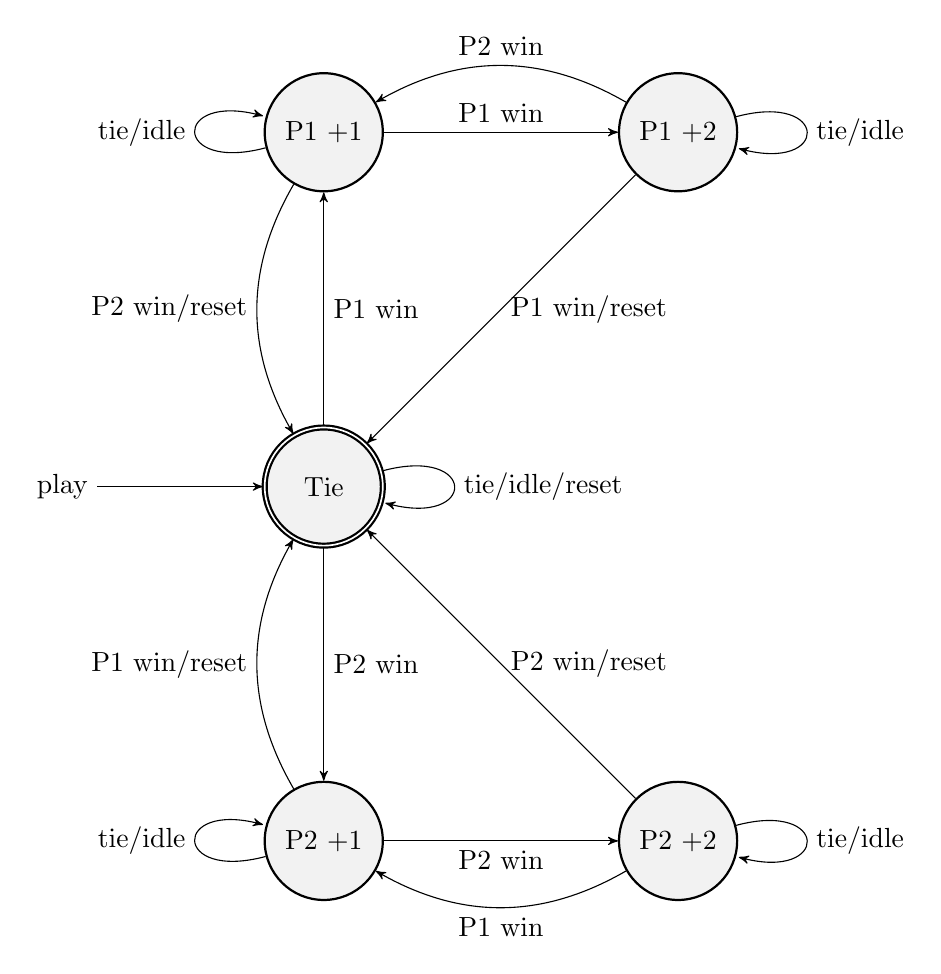
\begin{tikzpicture}
        % States definitions here
        % \node[<options>] (name) {text label};
        \node[state, initial, accepting, minimum size=1.5cm] (TIE) {Tie};
        \node[state, above of=TIE, minimum size=1.5cm] (P1_W1) {P1 +1};
        \node[state, below of=TIE, minimum size=1.5cm] (P2_W1) {P2 +1};
        \node[state, right of=P1_W1, minimum size=1.5cm] (P1_W2) {P1 +2};
        \node[state, right of=P2_W1, minimum size=1.5cm] (P2_W2) {P2 +2};

        % draw Edges
        % \draw (<source node>) edge[<edge options>] node[<node options>]{<edge label>} (<dest node>);
        \draw   (TIE)   edge[loop right] node[right]{tie/idle/reset} (TIE)
                        edge[] node[right]{P1 win} (P1_W1)
                        edge[] node[right]{P2 win} (P2_W1)
              
                (P1_W1) edge[bend right] node[left]{P2 win/reset} (TIE)
                        edge[loop left] node[]{tie/idle} (P1_W1)
                        edge[above] node[]{P1 win} (P1_W2)
              
                (P2_W1) edge[bend left] node[left]{P1 win/reset} (TIE)
                        edge[below] node[]{P2 win} (P2_W2)
                        edge[loop left] node[]{tie/idle} (P2_W1)
                        
                (P1_W2) edge[] node[right]{P1 win/reset} (TIE)
                        edge[loop right] node[]{tie/idle} (P1_W2)
                        edge[bend right] node[above]{P2 win} (P1_W1)

                (P2_W2) edge[] node[right]{P2 win/reset} (TIE)
                        edge[loop right] node[]{tie/idle} (P2_W2)
                        edge[bend left] node[below]{P1 win} (P2_W1)
                        ;
    \end{tikzpicture}
    \caption{Caption of the FSM}
\end{figure}



\end{document}
